% ------------------------------------------------------------------------
% ------------------------------------------------------------------------
% abnTeX2: Modelo de Trabalho Academico (tese de doutorado, dissertacao de
% mestrado e trabalhos monograficos em geral) em conformidade com 
% ABNT NBR 14724:2011: Informacao e documentacao - Trabalhos academicos -
% Apresentacao
%
% Adaptado por Emerson Ribeiro de Mello (2015-10-15)
% ------------------------------------------------------------------------
% ------------------------------------------------------------------------
\documentclass[
	% -- opções da classe memoir --
	12pt,				% tamanho da fonte
	openright,			% capítulos começam em pág ímpar (insere página vazia caso preciso)
	twoside,			% para impressão em verso e anverso. Oposto a oneside
	a4paper,			% tamanho do papel. 
	% -- opções da classe abntex2 --
	%chapter=TITLE,		% títulos de capítulos convertidos em letras maiúsculas
	%section=TITLE,		% títulos de seções convertidos em letras maiúsculas
	%subsection=TITLE,	% títulos de subseções convertidos em letras maiúsculas
	%subsubsection=TITLE,% títulos de subsubseções convertidos em letras maiúsculas
	% -- opções do pacote babel --
	english,			% idioma adicional para hifenização
%	french,				% idioma adicional para hifenização
%	spanish,			% idioma adicional para hifenização
	brazil				% o último idioma é o principal do documento
	]{abntex2}

%	Todas as indicações de pacotes e configurações estão no arquivo de estilo
%  chamado estilo-monografia-ifsc.sty.
\usepackage{estilo-monografia-ifsc}	
	

%---------------------------------------------------------------------%
%---------------------------------------------------------------------%
% Informações de dados para CAPA e FOLHA DE ROSTO
%---------------------------------------------------------------------%
%---------------------------------------------------------------------%
\titulo{Modelo de Trabalho Acadêmico com \abnTeX}
\autor{Nome do Aluno}
\local{São José - SC}
\data{outubro/2015}
\orientador{Professor Orientador da Silva}
\coorientador{Professor Coorientador da Silva}
\instituicao{%
  Instituto Federal de Santa Catarina -- IFSC
  \par
  Campus São José
  \par
  Engenharia de Telecomunicações}
\tipotrabalho{Monografia (Graduação)}

% O preambulo deve conter o tipo do trabalho, o objetivo, 
% o nome da instituição e a área de concentração 
\preambulo{Monografia apresentada à Coordenação de Engenharia de Telecomunicações do Instituto Federal de Santa Catarina para a obtenção do diploma Bacharel em Engenharia de Telecomunicações.}
%---------------------------------------------------------------------%








%---------------------------------------------------------------------%
% Início do documento
%---------------------------------------------------------------------%


\begin{document}
% Seleciona o idioma do documento (conforme pacotes do babel)
\selectlanguage{brazil}
% Retira espaço extra obsoleto entre as frases.
\frenchspacing 


% ----------------------------------------------------------
% ELEMENTOS PRÉ-TEXTUAIS
% ----------------------------------------------------------
% \pretextual

\imprimircapa
% Folha de rosto - (o * indica que haverá a ficha bibliográfica)
\imprimirfolhaderosto*
% ---

%---------------------------------------------------------------------%
% ATENÇÃO - Pergunte para a Biblioteca do IFSC
% Inserir a ficha bibliografica - 
%
%---------------------------------------------------------------------%
% Isto é um exemplo de Ficha Catalográfica, ou ``Dados internacionais de
% catalogação-na-publicação''. Você pode utilizar este modelo como referência. 
% Porém, provavelmente a biblioteca da sua universidade lhe fornecerá um PDF
% com a ficha catalográfica definitiva após a defesa do trabalho. Quando estiver
% com o documento, salve-o como PDF no diretório do seu projeto e substitua todo
% o conteúdo de implementação deste arquivo pelo comando abaixo:
%
% \begin{fichacatalografica}
%     \includepdf{fig_ficha_catalografica.pdf}
% \end{fichacatalografica}

\begin{fichacatalografica}
	\sffamily
	\vspace*{\fill}					% Posição vertical
	\begin{center}					% Minipage Centralizado
	\fbox{\begin{minipage}[c][8cm]{13.5cm}		% Largura
	\small
	\imprimirautor
	%Sobrenome, Nome do autor
	
	\hspace{0.5cm} \imprimirtitulo  / \imprimirautor. --
	\imprimirlocal, \imprimirdata-
	
	\hspace{0.5cm} \pageref{LastPage} p. : il. (algumas color.) ; 30 cm.\\
	
	\hspace{0.5cm} \imprimirorientadorRotulo~\imprimirorientador\\
	
	\hspace{0.5cm}
	\parbox[t]{\textwidth}{\imprimirtipotrabalho~--~\imprimirinstituicao,
	\imprimirdata.}\\
	
	\hspace{0.5cm}
		1. Palavra-chave1.
		2. Palavra-chave2.
		2. Palavra-chave3.
		I. Orientador.
		II. Instituto Federal de Santa Catarina.
		III. Campus São José.
		IV. Título 
	\end{minipage}}
	\end{center}
\end{fichacatalografica}
%---------------------------------------------------------------------%

%---------------------------------------------------------------------%
% Inserir folha de aprovação
%---------------------------------------------------------------------%

% Isto é um exemplo de Folha de aprovação, elemento obrigatório da NBR
% 14724/2011 (seção 4.2.1.3). Você pode utilizar este modelo até a aprovação
% do trabalho. Após isso, substitua todo o conteúdo deste arquivo por uma
% imagem da página assinada pela banca com o comando abaixo:
%
% \includepdf{folhadeaprovacao_final.pdf}
%
\begin{folhadeaprovacao}

  \begin{center}
    {\ABNTEXchapterfont\large\imprimirautor}

    \vspace*{\fill}\vspace*{\fill}
    \begin{center}
      \ABNTEXchapterfont\bfseries\Large\imprimirtitulo
    \end{center}
    \vspace*{\fill}
    
    \hspace{.45\textwidth}
    \begin{minipage}{.5\textwidth}
        \imprimirpreambulo
    \end{minipage}%
    \vspace*{\fill}
   \end{center}
        
   Trabalho aprovado. \imprimirlocal, 15 de outubro de 2015:

   \assinatura{\textbf{\imprimirorientador} \\ Orientador} 
   \assinatura{\textbf{Professor} \\ Convidado 1}
   \assinatura{\textbf{Professor} \\ Convidado 2}
   %\assinatura{\textbf{Professor} \\ Convidado 3}
   %\assinatura{\textbf{Professor} \\ Convidado 4}
      
   \begin{center}
    \vspace*{0.5cm}
    {\large\imprimirlocal}
    \par
    {\large\imprimirdata}
    \vspace*{1cm}
  \end{center}
  
\end{folhadeaprovacao}
% ---

%---------------------------------------------------------------------%
% Dedicatória
%---------------------------------------------------------------------%
\begin{dedicatoria}
   \vspace*{\fill}
   \centering
   \noindent
   \textit{ Este trabalho é dedicado às crianças adultas que,\\
   quando pequenas, sonharam em se tornar cientistas.} \vspace*{\fill}
\end{dedicatoria}
% ---

%---------------------------------------------------------------------%
% Agradecimentos
%---------------------------------------------------------------------%
\begin{agradecimentos}
Os agradecimentos principais são direcionados à Gerald Weber, Miguel Frasson,
Leslie H. Watter, Bruno Parente Lima, Flávio de Vasconcellos Corrêa, Otavio Real
Salvador, Renato Machnievscz\footnote{Os nomes dos integrantes do primeiro
projeto abn\TeX\ foram extraídos de
\url{http://codigolivre.org.br/projects/abntex/}} e todos aqueles que
contribuíram para que a produção de trabalhos acadêmicos conforme
as normas ABNT com \LaTeX\ fosse possível.

Agradecimentos especiais são direcionados ao Centro de Pesquisa em Arquitetura
da Informação\footnote{\url{http://www.cpai.unb.br/}} da Universidade de
Brasília (CPAI), ao grupo de usuários
\emph{latex-br}\footnote{\url{http://groups.google.com/group/latex-br}} e aos
novos voluntários do grupo
\emph{\abnTeX}\footnote{\url{http://groups.google.com/group/abntex2} e
\url{http://www.abntex.net.br/}}~que contribuíram e que ainda
contribuirão para a evolução do \abnTeX.

\end{agradecimentos}
% ---

%---------------------------------------------------------------------%
% Epígrafe
%---------------------------------------------------------------------%
\begin{epigrafe}
    \vspace*{\fill}
	\begin{flushright}
		\textit{``Não vos amoldeis às estruturas deste mundo, \\
		mas transformai-vos pela renovação da mente, \\
		a fim de distinguir qual é a vontade de Deus: \\
		o que é bom, o que Lhe é agradável, o que é perfeito.\\
		(Bíblia Sagrada, Romanos 12, 2)}
	\end{flushright}
\end{epigrafe}
% ---

%---------------------------------------------------------------------%
% RESUMOS
%---------------------------------------------------------------------%
% resumo em português
\setlength{\absparsep}{18pt} % ajusta o espaçamento dos parágrafos do resumo
\begin{resumo}
 Segundo a \citeonline[3.1-3.2]{NBR6028:2003}, o resumo deve ressaltar o
 objetivo, o método, os resultados e as conclusões do documento. A ordem e a extensão
 destes itens dependem do tipo de resumo (informativo ou indicativo) e do
 tratamento que cada item recebe no documento original. O resumo deve ser
 precedido da referência do documento, com exceção do resumo inserido no
 próprio documento. O resumo deve ser escrito como um parágrafo único, sem utilizar referências bibliográficas e evitando ao máximo, o uso de siglas/abreviações. O resumo deve conter até X palavras, sendo composto das seguintes partes (organização lógica): introdução, objetivos, justificativa, metodologia e resultados esperados. Esta é a sequência lógica, não devendo ser utilizados títulos e subtítulos. Não abuse na contextualização, pois o foco deve ser nos objetivos e nos resultados esperados. (\ldots) As palavras-chave devem figurar logo abaixo do
 resumo, antecedidas da expressão Palavras-chave:, separadas entre si por
 ponto e finalizadas também por ponto.

 \textbf{Palavras-chave}: latex. abntex. editoração de texto.
\end{resumo}

% resumo em inglês
\begin{resumo}[Abstract]
 \begin{otherlanguage*}{english}
   This is the english abstract.

   \vspace{\onelineskip}
 
   \noindent 
   \textbf{Keywords}: latex. abntex. text editoration.
 \end{otherlanguage*}
\end{resumo}


%---------------------------------------------------------------------%
% inserir lista de ilustrações, tabelas, listagem de códigos, abreviaturas, símbolos
%---------------------------------------------------------------------%
\pdfbookmark[0]{\listfigurename}{lof}
\listoffigures*
\cleardoublepage
% inserir lista de tabelas
\pdfbookmark[0]{\listtablename}{lot}
\listoftables*
\cleardoublepage
\newlistof{lstlistoflistings}{lol}{\lstlistlistingname}
\pdfbookmark[0]{\lstlistlistingname}{lol}
\lstlistoflistings*
\cleardoublepage

% inserir lista de abreviaturas e siglas
\pdfbookmark[0]{Lista de abreviaturas e siglas}{loa}
%%%%%%%%%%%%%% Como usar o pacote acronym
% \ac{acronimo} -- Na primeira vez que for citado o acronimo, o nome completo irá aparecer
%                  seguido do acronimo entre parênteses. Na proxima vez somente o acronimo
%                  irá aparecer. Se usou a opção footnote no pacote, entao o nome por extenso
%                  irá aparecer aparecer no rodapé
%
% \acf{acronimo} -- Para aparecer com nome completo + acronimo
% \acs{acronimo} -- Para aparecer somente o acronimo
% \acl{acronimo} -- Nome por extenso somente, sem o acronimo
% \acp{acronimo} -- igual o \ac mas deixando no plural com S (ingles)
% \acfp{acronimo}--
% \acsp{acronimo}--
% \aclp{acronimo}--

\chapter*{Lista de abreviaturas e siglas}%
% \addcontentsline{toc}{chapter}{Lista de abreviaturas e siglas}
\markboth{Lista de abreviaturas e siglas}{}


\begin{acronym}
	\acro{ABNT}{Associação Brasileira de Normas Técnicas}
	\acro{abnTeX}{ABsurdas Normas para TeX}
	\acro{AC}{Autoridade Certificadora}
	\acro{AES}{\textit{Advanced Encryption Standard}}
	\acro{TLS}{\textit{Transport Layer Security}}
	\acro{TPC}{Terceira Parte Confiável}
\end{acronym}



\cleardoublepage

% inserir lista de símbolos
\begin{simbolos}
  \item[$ \Gamma $] Letra grega Gama
  \item[$ \Lambda $] Lambda
  \item[$ \zeta $] Letra grega minúscula zeta
  \item[$ \in $] Pertence
\end{simbolos}
%---------------------------------------------------------------------%




%---------------------------------------------------------------------%
% inserir o sumario
%---------------------------------------------------------------------%
\pdfbookmark[0]{\contentsname}{toc}
\tableofcontents*
\cleardoublepage


% ----------------------------------------------------------
% ELEMENTOS TEXTUAIS
% ----------------------------------------------------------
\textual



% ----------------------------------------------------------
% Inclusão dos capítulos que estão em outros arquivos .tex
% ----------------------------------------------------------
% ----------------------------------------------------------------------- %
% Arquivo: introducao.tex
% ----------------------------------------------------------------------- %

\chapter{Introdução}
\label{c_introducao}

Neste capítulo serão introduzidos todos os assuntos abordados por este documento. Pretende-se apresentar a motivação, os objetivos e a organização do texto. A codificação de todos os arquivos do \abnTeX\ é \texttt{UTF8}. É necessário que você utilize a mesma codificação nos documentos que escrever, inclusive nos arquivos de base bibliográficas |.bib|.

É uma boa prática dividir o seu documento em diversos arquivos, e não apenas escrever tudo em um único. Esse recurso foi utilizado neste documento. Para incluir diferentes arquivos em um arquivo principal, de modo que cada arquivo incluído fique em uma página diferente, utilize o comando:

\begin{verbatim}
   \include{documento-a-ser-incluido}      % sem a extensão .tex
\end{verbatim}

Para incluir documentos sem quebra de páginas, utilize:

\begin{verbatim}
   \input{documento-a-ser-incluido}      % sem a extensão .tex
\end{verbatim}

% ---
\section{Compilar o documento \LaTeX}
% ---

Geralmente os editores \LaTeX, como o
TeXlipse\footnote{\url{http://texlipse.sourceforge.net/}}, o
Texmaker\footnote{\url{http://www.xm1math.net/texmaker/}}, entre outros,
compilam os documentos automaticamente, de modo que você não precisa se
preocupar com isso.

No entanto, você pode compilar os documentos \LaTeX usando os seguintes
comandos, que devem ser digitados no \emph{Prompt de Comandos} do Windows ou no
\emph{Terminal} do Mac ou do Linux:

\begin{verbatim}
   pdflatex ARQUIVO_PRINCIPAL.tex
   bibtex ARQUIVO_PRINCIPAL.aux
   makeindex ARQUIVO_PRINCIPAL.idx 
   makeindex ARQUIVO_PRINCIPAL.nlo -s nomencl.ist -o ARQUIVO_PRINCIPAL.nls
   pdflatex ARQUIVO_PRINCIPAL.tex
   pdflatex ARQUIVO_PRINCIPAL.tex
\end{verbatim}

% ---
\section{Referências bibliográficas}
% ---

A formatação das referências bibliográficas conforme as regras da ABNT são um
dos principais objetivos do \abnTeX. Consulte os manuais
\citeonline{abntex2cite} e \citeonline{abntex2cite-alf} para obter informações
sobre como utilizar as referências bibliográficas.

%-
\subsection{Acentuação de referências bibliográficas}
%-

Normalmente não há problemas em usar caracteres acentuados em arquivos
bibliográficos (\texttt{*.bib}). Porém, como as regras da ABNT fazem uso quase
abusivo da conversão para letras maiúsculas, é preciso observar o modo como se
escreve os nomes dos autores. Na ~\autoref{tabela-acentos} você encontra alguns
exemplos das conversões mais importantes. Preste atenção especial para `ç' e `í'
que devem estar envoltos em chaves. A regra geral é sempre usar a acentuação
neste modo quando houver conversão para letras maiúsculas.

\begin{table}[htbp]
\caption{Tabela de conversão de acentuação.}
\label{tabela-acentos}

\begin{center}
\begin{tabular}{ll}\hline\hline
acento & \textsf{bibtex}\\
à á ã & \verb+\`a+ \verb+\'a+ \verb+\~a+\\
í & \verb+{\'\i}+\\
ç & \verb+{\c c}+\\
\hline\hline
\end{tabular}
\end{center}
\end{table}




\section{Motivação}
\label{ci_s_motivacao}

A motivação deste documento foi a necessidade da elaboração de modelo para a concepção de monografias para o IFSC. 

\section{Organização do texto}
\label{ci_s_organizacao}

O texto está organizado da seguinte forma: No \autoref{c_cap2} é apresentado um pouco mais de como fazer um outro capítulo, apresentando ainda formas para inserir figuras. No \autoref{c_cap3} é apresentado uma forma para adicionar uma tabela. Por fim, no \autoref{c_conclusoes} são apresentadas as conclusões sobre este trabalho.
% ----------------------------------------------------------------------- %
% Arquivo: cap2.tex
% ----------------------------------------------------------------------- %

\chapter{Alguns conceitos}
\label{c_cap2}

Neste capítulo serão apresentadas formas para dividir o texto em seções e subseções bem como a inserção de figuras no texto. Será feito uso massivo de referências cruzadas para mostrar o poder do \LaTeX.

\section{A inclusão de figuras}
\label{s_c2_figuras}

As figuras são bastante úteis para ajudar expressar o funcionamento, modelo, etc. de alguma parte de seu trabalho. No Linux existem diversas aplicações para a criação de figuras, sendo o Xfig\footnote{\url{http://www.xfig.org}} uma ótima opção para a criação de figuras com alta qualidade, apesar de sua interface não ser muito amigável. Muitos utilizam outras aplicações com interfaces mais amigáveis e que ainda assim geram figuras com uma qualidade razoável como o \textit{Inkscape}, \textit{DIA}, \textit{OpenOffice Draw}, \textit{Kivio}, etc.

A inclusão de figuras no texto necessita que algumas regras sejam atendidas. São essas:

\begin{itemize}
	\item As figuras deverão ser de alta qualidade;
	\begin{itemize}
		\item Evite colocar fotos e outras figuras complexas;
		\item Opte por figuras simples e que realmente expressem algo, mesmo quando impressas em preto e branco;
	\end{itemize}
	\item Em \LaTeX as figuras deverão estar nos formatos: \texttt{PDF}, \texttt{JPG} ou \texttt{PNG};
	\item Toda figura deverá possuir uma legenda;
	\item Toda figura deverá ser referenciada em alguma parte do texto.
\end{itemize}

A \autoref{f_c2_disco} foi inserida no texto para mostrar como fazer tal inserção em \LaTeX. Vale lembrar que toda figura inserida deverá ser, em algum momento, referenciada no texto. 

\begin{figure}[!htpb]
	\centering
	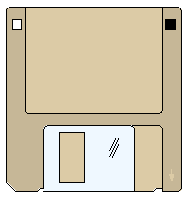
\includegraphics[width=5cm]{figs/disco}
	\caption{Disquete}
 	\label{f_c2_disco}
\end{figure}

O objetivo deste documento é de mostrar como preparar uma monografia para o Curso Superior de Tecnologia em Sistemas de Telecomunicações. No \autoref{c_cap3} é apresentado uma forma para fazer citações de outros trabalhos. O capítulo ainda apresenta uma forma para incluir tabelas no documento. O \autoref{c_conclusoes} apresenta as conclusões deste trabalho além de apresentar os trabalhos futuros.

\subsection{Mascotes}
\label{s_c2_mascotes}

Essa é uma subseção da \autoref{s_c2_figuras} do \autoref{c_cap2}. Subseções como esta não deverão ser numeradas. 

\begin{figure}[!htpb]
    \centering
    \begin{subfigure}[!htpb]{.45\textwidth}
        
\includegraphics[width=\textwidth]{figs/lion}
        \caption{O mascote estudando}
        \label{f_c2_masco1}
    \end{subfigure}
    \begin{subfigure}[!htpb]{.45\textwidth}
        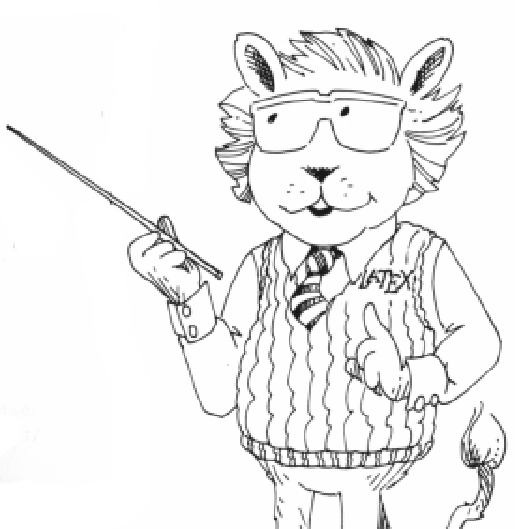
\includegraphics[width=\textwidth]{figs/latex_lion}
        \caption{O mascote ensinando}
        \label{f_c2_masco2}
    \end{subfigure}
	\caption{O mascote do \LaTeX em diferentes poses}
	\label{f_c2_mascotes}
\end{figure}

A \autoref{f_c2_mascotes} ilustra uma forma de incluir duas figuras, lado a lado. A \autoref{f_c2_masco1} ilustra o mascote do \LaTeX estudando. Já na \autoref{f_c2_masco2} o mascote aparece apresentando algum assunto. 


\section{Como apresentar equações}
\label{s_c2_equacoes}

O \LaTeX é um pacote feito para a preparação de textos impressos de alta qualidade, especialmente
para textos matemáticos. Ele foi desenvolvido por Leslie Lamport a partir do programa
\TeX criado por Donald Knuth.

Fórmulas matemáticas são produzidas digitando no arquivo fonte texto descrevendo-as. Isto
significa que o \LaTeX deve ser informado que o texto que vem a seguir é uma fórmula e também
quando ela termina e o texto normal recomeça. As fórmulas podem ocorrer em uma linha de
texto como $ax^2 + bx + c = 0$, ou destacada do texto principal como na \autoref{e_c2_eq1}.

\begin{equation}
 x=\frac{-b\pm\sqrt{b^2-4ac}}{2a}
\label{e_c2_eq1}
\end{equation}

\section{Incluindo trechos de códigos}

Em alguns casos é desejado incluir trechos de códigos no documento. O \LaTeX oferece inúmeras maneiras para isto e o pacote \textbf{listings} é conhecido por apresentar um dos melhores resultados. A \autoref{l_olamundo} apresenta o código em \textit{shell script} para o complexo problema do ``Olá mundo!''. A \autoref{l_matlab} apresenta um trecho de código em MatLab.

%parâmetros: linguagem (shell, java, matlab, python, c, php), label, caption, arquivo

\includecode[shell]{l_olamundo}{Olá mundo em shell script}{codigos/ola.sh}

\includecode[matlab]{l_matlab}{Um pequeno código em MatLab}{codigos/matlab.m}

% ---
\section{Divisões do documento: seção}\label{sec-divisoes}
% ---

Esta seção testa o uso de divisões de documentos. Esta é a
\autoref{sec-divisoes}. Veja a \autoref{sec-divisoes-subsection}.

\subsection{Divisões do documento: subseção}\label{sec-divisoes-subsection}

Isto é uma subseção. Veja a \autoref{sec-divisoes-subsubsection}, que é uma
\texttt{subsubsection} do \LaTeX, mas é impressa chamada de ``subseção'' porque
no Português não temos a palavra ``subsubseção''.

\subsubsection{Divisões do documento: subsubseção}
\label{sec-divisoes-subsubsection}

Isto é uma subsubseção.

\subsubsection{Divisões do documento: subsubseção}

Isto é outra subsubseção.

\subsection{Divisões do documento: subseção}\label{sec-exemplo-subsec}

Isto é uma subseção.

\subsubsection{Divisões do documento: subsubseção}

Isto é mais uma subsubseção da \autoref{sec-exemplo-subsec}.


\subsubsubsection{Esta é uma subseção de quinto
nível}\label{sec-exemplo-subsubsubsection}

Esta é uma seção de quinto nível. Ela é produzida com o seguinte comando:

\begin{verbatim}
\subsubsubsection{Esta é uma subseção de quinto
nível}\label{sec-exemplo-subsubsubsection}
\end{verbatim}

\subsubsubsection{Esta é outra subseção de quinto nível}\label{sec-exemplo-subsubsubsection-outro}

Esta é outra seção de quinto nível.


\paragraph{Este é um parágrafo numerado}\label{sec-exemplo-paragrafo}

Este é um exemplo de parágrafo nomeado. Ele é produzida com o comando de
parágrafo:

\begin{verbatim}
\paragraph{Este é um parágrafo nomeado}\label{sec-exemplo-paragrafo}
\end{verbatim}

A numeração entre parágrafos numeradaos e subsubsubseções são contínuas.

\paragraph{Esta é outro parágrafo numerado}\label{sec-exemplo-paragrafo-outro}

Esta é outro parágrafo nomeado.

% ---
\section{Este é um exemplo de nome de seção longo. Ele deve estar
alinhado à esquerda e a segunda e demais linhas devem iniciar logo abaixo da
primeira palavra da primeira linha}
% ---

Isso atende à norma \citeonline[seções de 5.2.2 a 5.2.4]{NBR14724:2011} 
 e \citeonline[seções de 3.1 a 3.8]{NBR6024:2012}.


\section{Usando siglas e abreviaturas}

Algumas vezes nos deparamos com textos cheios de siglas. O \LaTeX provê ferramentas para gerar glossário, lista de acrônimos, etc. Neste parágrafo é feito uso de comandos definidos no pacote \textit{acronym} e a listagem de acrônimos fica dentro do arquivo \texttt{abreviaturas.tex}.

O protocolo \ac{TLS} deve ser empregado sempre que se deseja garantir a integridade e a confidencialidade das mensagens trocadas pela rede. O \ac{TLS} é hoje utilizado por diversas aplicações. Como faz tempo que eu não falo do \acf{TLS} eu chamo o nome completo mais a sigla, ajudando o meu leitor a lembrar da sigla \ac{TLS}. Existe a \ac{AC} que é bem importante. Este documento segue as normas da \ac{ABNT} e para isso faz uso do pacote \ac{abnTeX}.


% ----------------------------------------------------------------------- %
% Arquivo: cap3.tex
% ----------------------------------------------------------------------- %
\chapter{Conceitos finais sobre o documento}
\label{c_cap3}

Neste capítulo, diferentemente do ocorreu na \autoref{s_c2_figuras} do \autoref{c_cap2}, será apresentado uma forma para inserir tabelas no documento. A \autoref{t_c3_etapas} é só um pequeno exemplo de tabela.

\begin{table}[!htpb]
% \ABNTEXfontereduzida
\centering
\caption{Cronograma das atividades previstas}
\label{t_c3_etapas}
 \setlength{\tabcolsep}{3pt}
\begin{tabular}{|c|c|c|c|c|c|c|c|c|c|c|c|c|}\hline
 & \multicolumn{12}{c|}{Semanas}\\ \cline{2-13}
\raisebox{1.5ex}{Etapa} & 01 & 02 & 03 & 04 & 05 & 06 & 07 & 08 & 09 & 10 & 11 & 12 \\ \hline
1 & $\surd$ & $\surd$ & $\surd$ & & & & & & & & & \\ \hline
2 & & & & $\surd$ & $\surd$ & $\surd$ & $\surd$ & & & & & \\ \hline
3 & & & & & & & & $\surd$ & $\surd$ & $\surd$ & & \\ \hline
4 & & & & & & & & & & & $\surd$ & $\surd$ \\ \hline
\end{tabular} 
\end{table} 

\index{tabelas}A \autoref{tab-nivinv} é um exemplo de tabela construída em \LaTeX.

\begin{table}[htb]
\ABNTEXfontereduzida
\caption[Níveis de investigação]{Níveis de investigação.}
\label{tab-nivinv}
\begin{tabular}{p{2.6cm}|p{6.0cm}|p{2.25cm}|p{3.40cm}}
  %\hline
   \textbf{Nível de Investigação} & \textbf{Insumos}  & \textbf{Sistemas de Investigação}  & \textbf{Produtos}  \\
    \hline
    Meta-nível & Filosofia\index{filosofia} da Ciência  & Epistemologia &
    Paradigma  \\
    \hline
    Nível do objeto & Paradigmas do metanível e evidências do nível inferior &
    Ciência  & Teorias e modelos \\
    \hline
    Nível inferior & Modelos e métodos do nível do objeto e problemas do nível inferior & Prática & Solução de problemas  \\
   % \hline
\end{tabular}
\legend{Fonte: \citeonline{van86}}
\end{table}

Já a \autoref{tabela-ibge} apresenta uma tabela criada conforme o padrão do \citeonline{ibge1993} requerido pelas normas da ABNT para documentos técnicos e acadêmicos.

\begin{table}[htb]
\IBGEtab{%
  \caption{Um Exemplo de tabela alinhada que pode ser longa
  ou curta, conforme padrão IBGE.}%
  \label{tabela-ibge}
}{%
  \begin{tabular}{ccc}
  \toprule
   Nome & Nascimento & Documento \\
  \midrule \midrule
   Maria da Silva & 11/11/1111 & 111.111.111-11 \\
  \midrule 
   João Souza & 11/11/2111 & 211.111.111-11 \\
  \midrule 
   Laura Vicuña & 05/04/1891 & 3111.111.111-11 \\
  \bottomrule
\end{tabular}%
}{%
  \fonte{Produzido pelos autores.}%
  \nota{Esta é uma nota, que diz que os dados são baseados na
  regressão linear.}%
  \nota[Anotações]{Uma anotação adicional, que pode ser seguida de várias
  outras.}%
  }
\end{table}



\section{Como usar referências bibliográficas}
\label{s_c3_referencias}

O uso de citações ao londo do texto é uma prática desejável. Por exemplo, em \cite{lamport94} é apresentado um documento sobre a preparação de textos usando \LaTeX. Já em \cite{goossens94} é apresentada uma lista de referências rápidas para realizar as mais simples tarefas em \LaTeX.

É o caso em que você menciona \emph{explicitamente} o autor da referência na sentença, algo
do tipo ``Fulano (1900)''. Neste caso o nome do autor é escrito
normalmente. Para isso use o comando \verb+\citeonline+.

A ironia será assim uma \ldots\ proposta  por \citeonline{lamport94}. Em \cite{exemplo} foi usado para ilustrar como uma \textit{URL} deve aparecer na seção das referências. Este documento segue as normas da \ac{ABNT} e para isso faz uso do pacote \ac{abnTeX}.


% ---
\section{Citações diretas}
\label{sec-citacao}
% ---

\index{citações!diretas}Utilize o ambiente \texttt{citacao} para incluir
citações diretas com mais de três linhas:

\begin{citacao}
As citações diretas, no texto, com mais de três linhas, devem ser
destacadas com recuo de 4 cm da margem esquerda, com letra menor que a do texto
utilizado e sem as aspas. No caso de documentos datilografados, deve-se
observar apenas o recuo \cite[5.3]{NBR10520:2002}.
\end{citacao}

Use o ambiente assim:

\begin{verbatim}
\begin{citacao}
As citações diretas, no texto, com mais de três linhas [...] deve-se observar
apenas o recuo \cite[5.3]{NBR10520:2002}.
\end{citacao}
\end{verbatim}

O ambiente \texttt{citacao} pode receber como parâmetro opcional um nome de
idioma previamente carregado nas opções da classe. Nesse
caso, o texto da citação é automaticamente escrito em itálico e a hifenização é
ajustada para o idioma selecionado na opção do ambiente. Por exemplo:

\begin{verbatim}
\begin{citacao}[english]
Text in English language in italic with correct hyphenation.
\end{citacao}
\end{verbatim}

Tem como resultado:

\begin{citacao}[english]
Text in English language in italic with correct hyphenation.
\end{citacao}

\index{citações!simples}Citações simples, com até três linhas, devem ser
incluídas com aspas. Observe que em \LaTeX as aspas iniciais são diferentes das
finais: ``Amor é fogo que arde sem se ver''.







% ----------------------------------------------------------------------- %
% Arquivo: conclusoes.tex
% ----------------------------------------------------------------------- %

\chapter{Conclusões}
\label{c_conclusoes}

Este trabalho procurou mostrar como deverá ser a apresentação da monografia a ser submetida à Coordenação do Curso de Engenharia de Telecomunicações do Instituto Federal de Santa Catarina para a obtenção do diploma de Bacharel em Engenharia de Telecomunicações.

No \autoref{c_introducao} foi feita uma pequena introdução. No \autoref{c_cap2} foram apresentados alguns comentários sobre figuras. E no \autoref{c_cap3} foi apresentada uma forma para inserir tabela.

Como trabalho futuro, fica a reescrita do texto deste documento de forma que ele possam indicar informações específicas a formatação do documento. Como o tamanho da fonte utilizada, o espaçamento da borda, o alinhamento e numeração das seções e capítulos, etc.






% ----------------------------------------------------------
% ELEMENTOS PÓS-TEXTUAIS
% ----------------------------------------------------------
\postextual
% ----------------------------------------------------------

% ----------------------------------------------------------
% Referências bibliográficas
% ----------------------------------------------------------
\bibliography{referencias}


% ----------------------------------------------------------
% Apêndices
% ----------------------------------------------------------
\begin{apendicesenv}
% Imprime uma página indicando o início dos apêndices
\partapendices

\chapter{Meu primeiro apêndice}
\lipsum[50]

\end{apendicesenv}

% ----------------------------------------------------------
% Anexos
% ----------------------------------------------------------
\begin{anexosenv}
% Imprime uma página indicando o início dos anexos
\partanexos

\chapter{Meu primeiro assunto de anexo}
\lipsum[30]


\chapter{Segundo assunto que pesquisei}
\lipsum[31]

\end{anexosenv}

%---------------------------------------------------------------------
% INDICE REMISSIVO
%---------------------------------------------------------------------
\phantompart
\printindex
%---------------------------------------------------------------------

\end{document}
